\documentclass{beamer}

\usetheme{Antibes}

% Loading preambulo
% PREAMBULO ====================================================================

% Packages ---------------------------------------------------------------------

% Package to Portuguese language
\usepackage[brazilian]{babel}
% Packages to Figures
\usepackage{graphicx}
\usepackage{tikz}
% Packages to math symbols and expressions
\usepackage{amsfonts, amssymb, amsmath}
% Packages to insert code
\usepackage{listings} 
\usepackage{verbatim}
% Package to justify text
\usepackage[document]{ragged2e}
% Package to manage the bibliography
\usepackage[backend=biber, style=numeric, sorting=none]{biblatex}
% Package to facilitate quotations
\usepackage{csquotes}
% Package to use multicols
\usepackage{multicol}
% Packages for url
%	The package libertinus already loads hyperref
%\usepackage[colorlinks=true]{hyperref}
% Font
%   Fira
%\usepackage[sfdefault, lf]{FiraSans}
%   Libertinus
\usepackage{libertinus}
\renewcommand*\familydefault{\sfdefault} %% Only if the base font of the document is to be sans serif
% Colors
\usepackage{xcolor}
\usepackage{colortbl}
% Table
\usepackage{tabularray}
% Fill line
\usepackage{xhfill}

% Configurations ---------------------------------------------------------------

\AtBeginSection{
    \begin{frame}{\secname}
        \tableofcontents[currentsection,hideallsubsections]
    \end{frame}
}

\AtBeginSubsection{
    \begin{frame}{\subsecname}
        \tableofcontents[currentsection,subsectionstyle=show/shaded/hide, subsubsectionstyle=hide]
    \end{frame}
}

\AtBeginSubsubsection{
    \begin{frame}{\subsubsecname}
        \tableofcontents[currentsection,subsectionstyle=show/shaded/hide,subsubsectionstyle=show/shaded/hide/hide]
    \end{frame}
}

% Numbering slides
\setbeamertemplate{footline}[frame number]{}

% Getting rid of bottom navigation bars
\setbeamertemplate{navigation symbols}{}

% Margins
\setbeamersize{text margin left=20pt, text margin right=20pt}

% Colors
\definecolor{burgundy}{RGB}{133,24,42}
\definecolor{bloodred}{RGB}{147,5,5}

\setbeamercolor{structure}{fg=burgundy}

\setbeamercolor*{palette primary}{use=structure,fg=white,bg=structure.fg}
%\setbeamercolor*{palette secondary}{use=structure,fg=white,bg=structure.fg!75!black}
%\setbeamercolor*{palette tertiary}{use=structure,fg=white,bg=structure.fg!50!black}
\setbeamercolor*{palette quaternary}{fg=white,bg=bloodred}

%	hyperref
\hypersetup{
	colorlinks=true,
	urlcolor=blue,
	breaklinks=true}

% New commands -----------------------------------------------------------------

\NewTblrTableCommand \aula{\SetCell{bg=green!60,fg=white}}
\NewTblrTableCommand \prova{\SetCell{bg=red!80,fg=white}}
\NewTblrTableCommand \feriado{\SetCell{bg=blue!50,fg=white}}

\newcommand{\esta}[1]{\textbf{\underline{#1}}}

% Title
\title[GP 04]{Gerência de Projetos}
% Subtitle
\subtitle{Aula 04}
% Author of the presentation
\author[E.J.R. Silva]{Evandro J.R. Silva}
% date of the presentation
\date{}

\begin{document}
    
\begin{frame}
    \titlepage
\end{frame}

\begin{frame}{Sumário}
    \tableofcontents
\end{frame}

%===============================================================================
% SECTION 1 ====================================================================
%===============================================================================
\section{Domínios de desempenho de projetos}

\begin{frame}{Domínios de desempenho de projetos}
    \begin{itemize}
        \justifying
        \item<1-> Um domínio de desempenho do projeto é um \textbf{grupo de atividades relacionadas}, que são \textbf{críticas para a entrega eficaz dos resultados} do projeto.
        \item<2-> Os domínios de desempenho de projetos
        	\begin{itemize}
        		\justifying
        		\item<2-> São \textbf{áreas de foco interativas}, \textbf{inter-relacionadas} e \textbf{interdependentes} que trabalham em uníssono \textbf{para alcançar os resultados desejados do projeto}.
        		\item<3-> \textbf{São executados simultaneamente ao longo do projeto}, independentemente de como o valor seja entregue.
        	\end{itemize}
        \item<4> As \textbf{atividades específicas realizadas em cada um dos domínios} de desempenho \textbf{são determinadas pelo contexto da organização}, \textbf{o projeto}, \textbf{as entregas}, \textbf{a equipe do projeto}, \textbf{as partes interessadas} e outros fatores.
    \end{itemize}
\end{frame}

\begin{frame}{Domínios de desempenho de projetos}
	\begin{itemize}
		\item Existem oito domínios de desempenho de projetos
			\begin{itemize}
				\item Partes interessadas.
				\item Equipe.
				\item Abordagem de desenvolvimento e ciclo de vida.
				\item Planejamento.
				\item Trabalho do projeto.
				\item Entrega.
				\item Medição.
				\item Incerteza.
			\end{itemize}
	\end{itemize}
\end{frame}

%-------------------------------------------------------------------------------
% SUBSECTION 1.1 ---------------------------------------------------------------
%-------------------------------------------------------------------------------
\subsection{Partes interessadas}

\begin{frame}{Partes interessadas}
	\begin{itemize}
		\justifying
		\small
		\item Envolve engajar e trabalhar com as partes interessadas para promover relacionamentos positivos e a satisfação.
		\item Para isso são muito importantes as habilidades interpessoais e de liderança.
	\end{itemize}
	\vspace{5pt}
	\centering
	
\includegraphics[width=\textwidth]{imagens/figura01.png}
\end{frame}

%-------------------------------------------------------------------------------
% SUBSECTION 1.2 ---------------------------------------------------------------
%-------------------------------------------------------------------------------
\subsection{Equipe}

\begin{frame}{Equipe}
	\begin{itemize}
		\justifying
		\item Envolve estabelecer a cultura e o ambiente que permitem que um grupo de diversos indivíduos evolua para uma equipe de projeto de alto desempenho.
	\end{itemize}
	\vspace{5pt}
	\centering
	
\includegraphics[width=\textwidth]{imagens/figura02.png}
\end{frame}

%-------------------------------------------------------------------------------
% SUBSECTION 1.3 ---------------------------------------------------------------
%-------------------------------------------------------------------------------
\subsection{Abordagem de desenvolvimento e ciclo de vida}

\begin{frame}{Abordagem de desenvolvimento e ciclo de vida}
	\begin{itemize}
		\justifying
		\item Envolve o estabelecimento da abordagem de desenvolvimento, cadência de entrega e ciclo de vida do projeto necessários para otimizar os resultados do projeto.
	\end{itemize}
	\vspace{5pt}
	\centering
	
\includegraphics[width=\textwidth]{imagens/figura03.png}
\end{frame}

%-------------------------------------------------------------------------------
% SUBSECTION 1.4 ---------------------------------------------------------------
%-------------------------------------------------------------------------------
\subsection{Planejamento}

\begin{frame}{Planejamento}
	\begin{itemize}
		\justifying
		\item O planejamento organiza, elabora e coordena o trabalho do projeto, durante todo o projeto.
	\end{itemize}
	\vspace{5pt}
	\centering
	
\includegraphics[width=0.8\textwidth]{imagens/figura04.png}
\end{frame}

%-------------------------------------------------------------------------------
% SUBSECTION 1.5 ---------------------------------------------------------------
%-------------------------------------------------------------------------------
\subsection{Trabalho do projeto}

\begin{frame}{Trabalho do projeto}
	\begin{itemize}
		\justifying
		\item Está associado ao estabelecimento dos processos e à execução do trabalho para permitir que a equipe do projeto gere as entregas e os resultados esperados.
	\end{itemize}
	\vspace{5pt}
	\centering
	
\includegraphics[width=0.9\textwidth]{imagens/figura05.png}
\end{frame}

%-------------------------------------------------------------------------------
% SUBSECTION 1.6 ---------------------------------------------------------------
%-------------------------------------------------------------------------------
\subsection{Entrega}

\begin{frame}{Entrega}
	\begin{itemize}
		\justifying
		\item Concentra-se em atender aos requisitos, escopo e expectativas de qualidade para produzir as entregas esperadas que conduzirão aos resultados pretendidos.
	\end{itemize}
	\vspace{5pt}
	\centering
	
\includegraphics[width=0.9\textwidth]{imagens/figura06.png}
\end{frame}


%-------------------------------------------------------------------------------
% SUBSECTION 1.7 ---------------------------------------------------------------
%-------------------------------------------------------------------------------
\subsection{Medição}

\begin{frame}{Medição}
	\begin{itemize}
		\justifying
		\item Avalia o grau em que o trabalho realizado no domínio de desempenho da entrega está cumprindo as métricas identificadas no domínio de desempenho do planejamento.
	\end{itemize}
	\vspace{5pt}
	\centering
	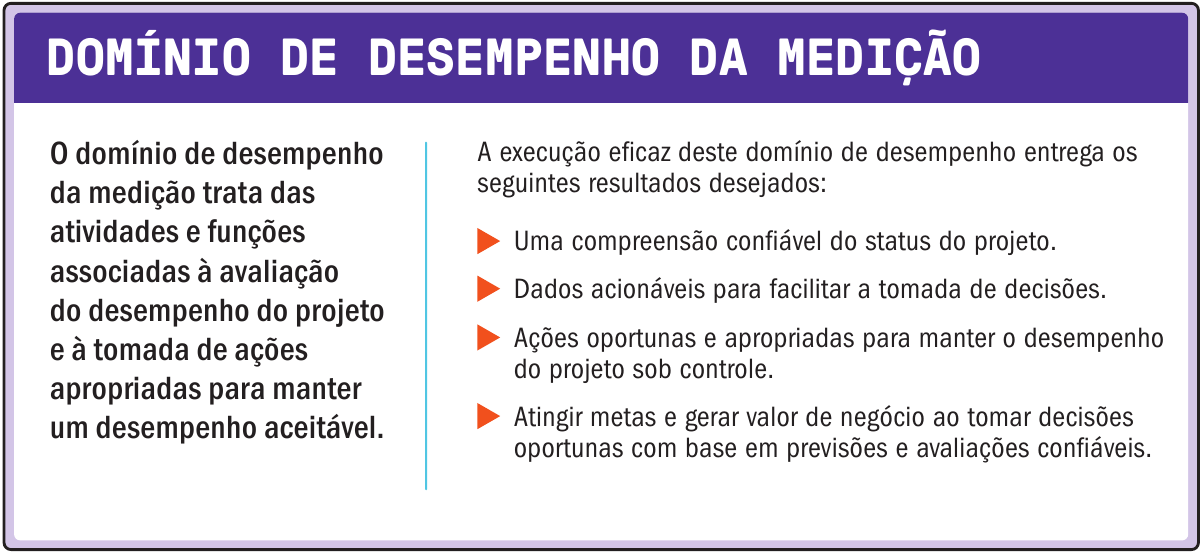
\includegraphics[width=\textwidth]{imagens/figura07.png}
\end{frame}

%-------------------------------------------------------------------------------
% SUBSECTION 1.8 ---------------------------------------------------------------
%-------------------------------------------------------------------------------
\subsection{Incerteza}

\begin{frame}{Incerteza}
	\begin{itemize}
		\justifying
		\item Aborda os vários aspectos da incerteza, suas implicações, como o risco do projeto, bem como as opções para navegar pelas várias formas de incerteza.
	\end{itemize}
\end{frame}

\begin{frame}{Incerteza}
	\centering
	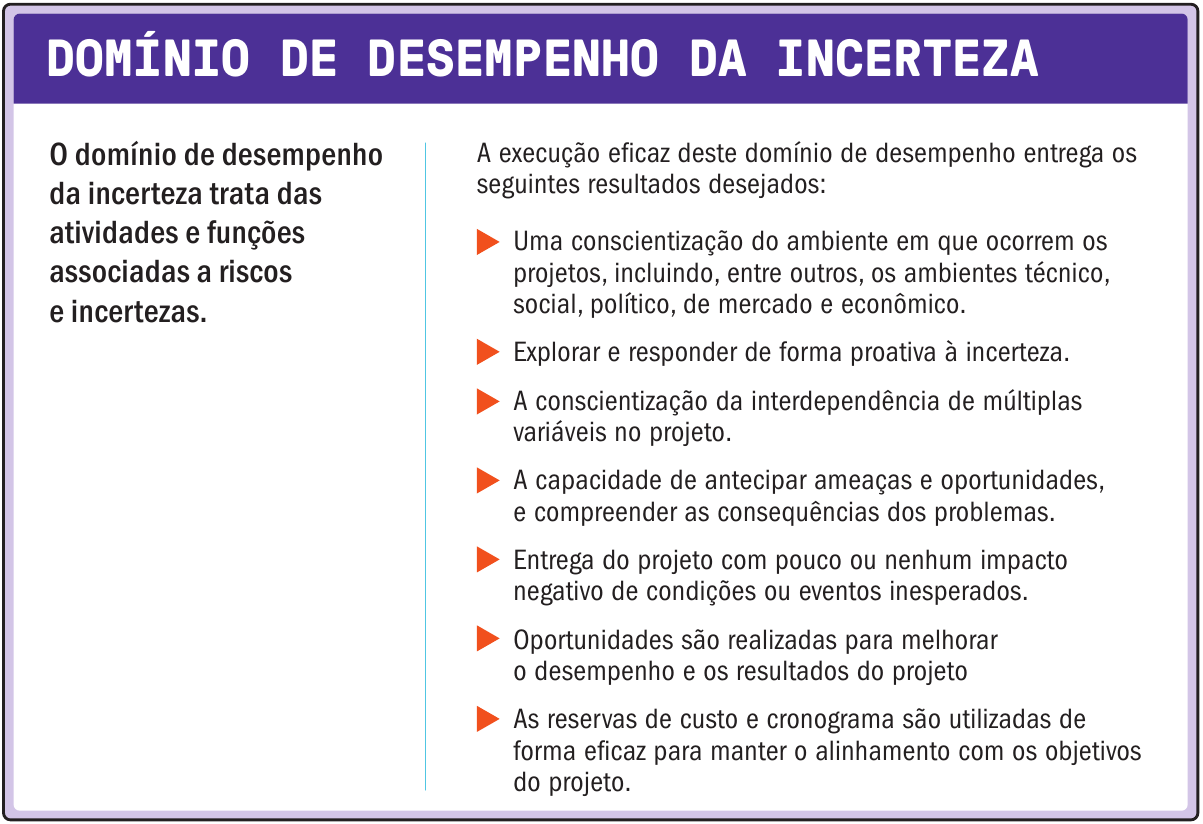
\includegraphics[width=0.9\textwidth]{imagens/figura08.png}
\end{frame}

%===============================================================================
% SECTION 2 ====================================================================
%===============================================================================
\section{Atividade}

\begin{frame}{Atividade}
    \begin{itemize}
        \justifying
        \item Dividam-se em grupos. Cada grupo receberá um ou mais domínios, sobre os quais deverão estudar o conteúdo presente no PMBOK, principalmente a seção \textbf{Verificação de Resultados}.
        \item Para cada domínio, um cenário fictício será apresentado, e o grupo deve explicar a importância do seu domínio para o projeto do respectivo cenário.
    \end{itemize}
\end{frame}

\begin{frame}{Atividade}
	\begin{itemize}
		\item Cenários
			\begin{itemize}
				\justifying
				\item \textbf{Partes interessadas}: O projeto é a construção de uma usina solar. A tecnologia é perfeita e o financiamento está garantido, mas a comunidade local e uma ONG ambiental entraram com uma liminar para paralisar as obras por falta de diálogo.
				\item \textbf{Equipe}: Uma equipe de alto nível técnico está trabalhando em silos. O clima é de desconfiança, as informações não circulam e dois desenvolvedores chave pediram demissão por burnout.
				\item \textbf{Abordagem de Desenvolvimento e Ciclo de Vida}: Uma empresa de varejo quer lançar um super-app. Metade da diretoria quer o método Cascata (para saber o custo total logo) e a outra metade quer Ágil (para lançar logo). O projeto está travado na indecisão.
				\item \textbf{Planejamento}: O projeto sofreu uma redução de 30\% no orçamento no meio da execução. O cronograma original agora é impossível de cumprir com os recursos atuais.
			\end{itemize}
	\end{itemize}
\end{frame}

\begin{frame}{Atividade}
	\begin{itemize}
		\item Cenários
		\begin{itemize}
			\justifying
			\item \textbf{Trabalho do Projeto}: O fluxo de trabalho está lento. Há excesso de burocracia, reuniões improdutivas e a equipe gasta mais tempo preenchendo relatórios do que produzindo as entregas.
			\item \textbf{Entrega}: O projeto entregou todas as funcionalidades solicitadas no escopo inicial, mas o cliente final não está usando o produto porque ele não resolve o problema atual do mercado.
			\item \textbf{Medição}: O projeto tem centenas de indicadores, mas ninguém sabe se o projeto está indo bem ou mal. Os dados são contraditórios e a diretoria está confusa.
			\item \textbf{Incerteza}: Um projeto de inovação tecnológica enfrenta uma crise global de chips e mudanças súbitas na legislação tributária. O risco de fracasso é de 70\%.
		\end{itemize}
	\end{itemize}
\end{frame}

\begin{frame}{Atividade}
	\begin{itemize}
		\item Desafios
		\begin{itemize}
			\justifying
			\item \textbf{Partes Interessadas}: Por que gastar tempo e dinheiro com `gestão de expectativas' se o contrato já foi assinado e temos o direito legal de construir? O foco não deveria ser apenas na execução técnica?
			\item \textbf{Equipe}: Em um projeto com prazo apertado, como você justifica investir horas em `desenvolvimento de equipe' e `cultura' em vez de simplesmente contratar substitutos e exigir que trabalhem mais rápido?
			\item \textbf{Abordagem de Desenvolvimento e Ciclo de Vida}: Se o mercado muda a cada mês, por que perder tempo definindo um `Ciclo de Vida' agora? Não seria melhor apenas começar a programar e ver o que acontece?
			\item \textbf{Planejamento}: Se o planejamento nunca sobrevive ao primeiro contato com a realidade e tudo mudou, por que ele ainda é considerado um domínio de desempenho e não uma perda de tempo burocrática?
		\end{itemize}
	\end{itemize}
\end{frame}

\begin{frame}{Atividade}
	\begin{itemize}
		\item Desafios
		\begin{itemize}
			\justifying
			\item \textbf{Trabalho do Projeto}: Como você prova que `gerenciar o trabalho' (processos) agrega mais valor do que focar 100\% na `entrega final' do produto?
			\item \textbf{Entrega}: Se o escopo foi 100\% cumprido, o domínio de Entrega foi um sucesso? Como você defende esse domínio quando o `sucesso' técnico não gera `valor' de negócio?
			\item \textbf{Medição}: Medir custa caro e gera ansiedade na equipe. Por que não confiamos apenas no `sentimento' do gerente de projeto experiente em vez de gastar com softwares complexos de dashboard?
			\item \textbf{Incerteza}: Se a incerteza é algo que não podemos controlar, por que não aceitamos o caos e reagimos apenas quando os problemas aparecerem, em vez de gastar energia com `planos de resposta a riscos' que podem nunca ocorrer?
		\end{itemize}
	\end{itemize}
\end{frame}

%===============================================================================
% FIM ==========================================================================
%===============================================================================

\begin{frame}
    \centering
    \Large
    FIM
\end{frame}
    
\end{document}
